\section{Constraints}
constraints in design and implementation

\subsection{Riot API Ratelimits}

\subsection{Server Performance}

Als Infrastruktur wurde der Landesdienst von bwCloud verwendet, der eine kostenlose
"Infrastructure-as-a-Service" Umgebung für Forschung und Lehre in Baden-Württemberg bereitstellt.
Wie Grafik \ref{fig:uebersicht_kontingente} zeigt, kann pro Nutzer nur ein bestimmtes Kontingent an VCPUS, RAM sowie Datenträger-Speicher verwendet werden.
Sobald mehr Server-Ressourcen benötigt werden, ist dies nicht möglich ohne auf einen kostenpflichtigen Dienst wechseln zu müssen.

\begin{figure}
\centering
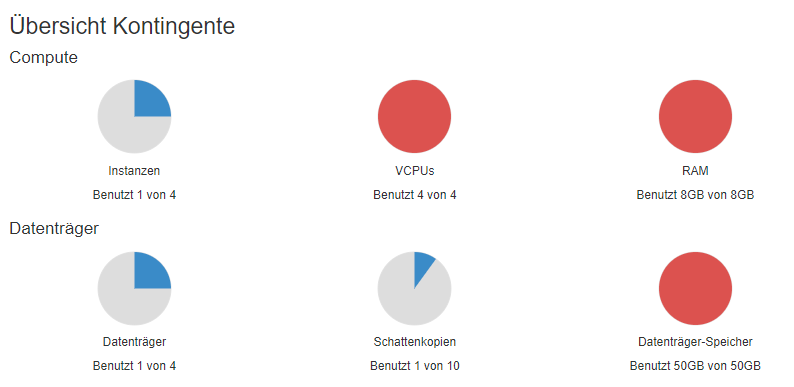
\includegraphics[width=0.8\textwidth]{uebersicht_kontingente.png}
\caption{Übersicht der verfügbaren Kontigente}
\label{fig:uebersicht_kontingente}
\end{figure}

Diese beschränkten Ressourcen haben einen direkten Einfluss auf die Ausführung von komplexen Datenbankoperationen. Außerdem ist ein
horizontales Scaling des Dienstes durch die Limitierung ebenso nicht möglich, wodurch nur die Performance durch verbesserte SQL-Abfragen
optimiert werden kann.
